\appendix
\chapter{Anlagen}
\section{Well-Known-Binary Format (WKB)}
\label{sec:appendix:wkb}
Das \textit{Well-Known-Binary} Format ist die binäre Repräsentation eines geometrischen Objekts des \textit{Simple Feature Models}.
Dieses Modell ist eine Untermenge des ISO 19107 Standards, welcher die geometrischen Eigenschaften von Geoobjekten spezifiziert. Ausgehend von einer allgemeinen Oberklasse können geometrische Primitive, wie z.B. ein Punkt, oder komplexe geometrische Objekte, wie z.B. Flächen oder Sammlungen von Objekten, beschrieben werden. (vgl. \cite{Bill2010}:358ff.). Die verfügbaren Klassen werden in Abbildung \ref{fig:bill_sfm} aufgezeigt.
\begin{figure}[!htb]
  \centering
   \fbox{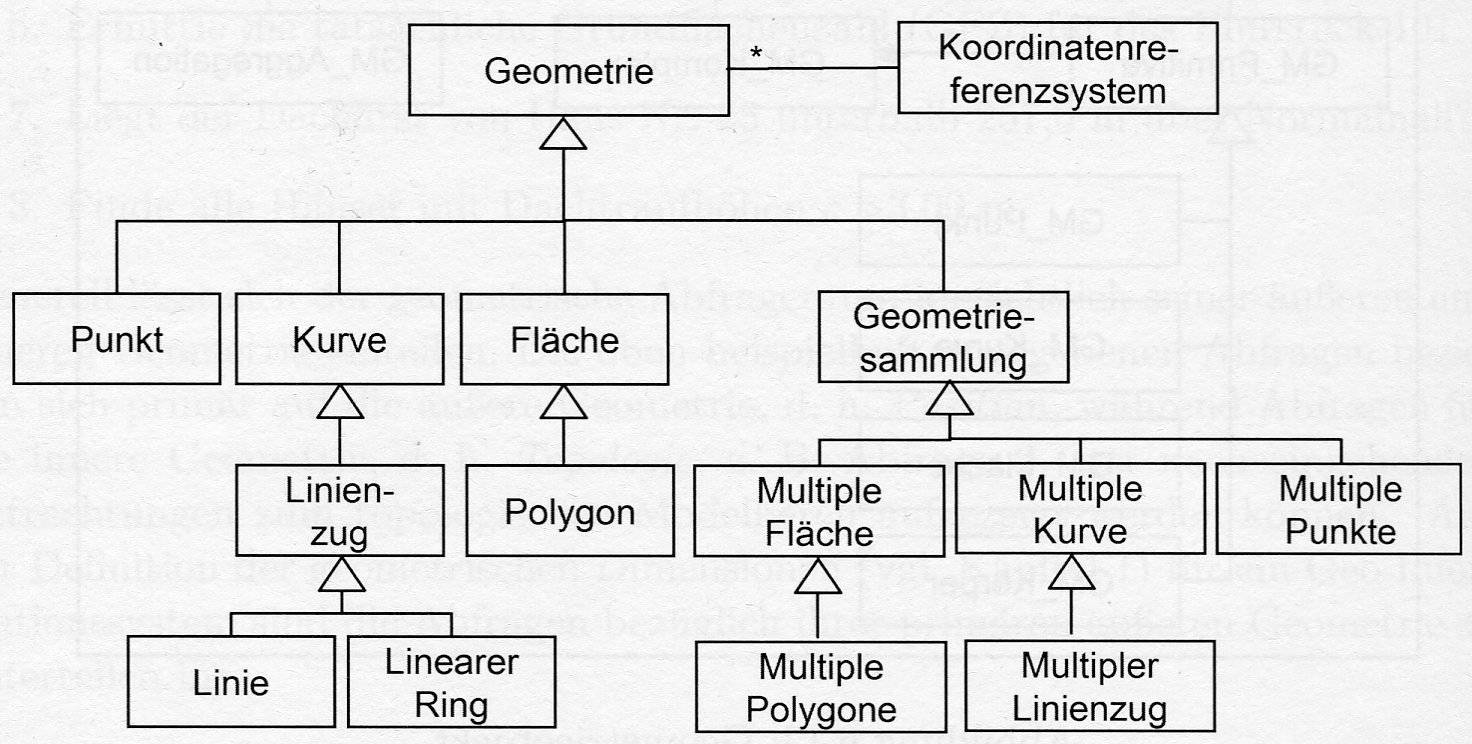
\includegraphics[width=1\textwidth]{gfx/bill_sfm001.jpg}}
   \caption{Geometrien im Simple Feature Model \protect\cite{Bill2010}:360}
   \label{fig:bill_sfm}
\end{figure}

Das WKB Format wird beispielsweise innerhalb der PostgreSQL Erweiterung PostGIS\footnote{http://postgis.net} genutzt, um geometrische Objekte in einer Datenbank abzulegen.
Analog dazu existiert das \textit{Well-Known-Text} Format, welches die textuelle Repräsentation geometrischer Objekte des Simple Feature Models spezifiziert.

\subsubsection{Beispiel für das WKB und das WKT Format}
Ein Punkt mit den Koordinaten \texttt{13.439561 Ost} sowie \texttt{52.54002 Nord} entspricht der WKT Repräsentation\\\\
\texttt{SRID=4326;POINT(13.439561 52.54002)}\\\\
und\\\\
\texttt{0101000020E6100000B131AF230EE12A40CC9717601F454A40}\\\\
in der WKB Repräsentation.

Der Wert \texttt{SRID} beinhaltet die ID des zu verwendenden Koordinatenreferenzsystems.
Die ID \texttt{4326} entspricht dem häufig verwendeten Referenzsystem \texttt{WGS84}\footnote{http://spatialreference.org/ref/epsg/4326/}.  

\section{GeoJSON}
\label{sec:appendix:geojson}
GeoJSON\footnote{http://geojson.org} ist ein Format zur Repräsentation von geometrischen Objekten im JSON Format.
Es verwendet ein ähnliches hierarchisches Klassenmodell. (vgl. \cite{WEB:GEOJSON:Spec:2008}).

\subsubsection{Beispiel für das GeoJSON Format}
Ein Beispiel der GeoJSON Repräsentation eines Punktes mit den Koordinaten \texttt{13.439561 Ost} sowie \texttt{52.54002 Nord} ist in Listing \ref{example_geojson} ersichtlich.
\lstset{
  numbers=none,
  caption=Beispiel eines geometrischen Punktes in GeoJSON Repräsentation,
  label=example_geojson
}
\begin{lstlisting}
  {
    "type": "Point",
    "coordinates": [
        13.439561,
        52.54002
    ]
}
\end{lstlisting}

\section{OpenStreetMap Datenformat}
\label{sec:appendix:osm:data}
OpenStreetMap bietet seine Daten zum Download in einer Datei namens \textit{planet.osm}\footnote{http://planet.openstreetmap.org/} an. Diese Datei im XML-Format enthält den kompletten Datenbestand des OpenStreetMap Projekts. 
Da diese Datei sehr groß ist (gepackt ca. 50GB) bieten andere Dienstleister, wie zum Beispiel die Geofabrik GmbH Karlsruhe\footnote{http://www.geofabrik.de}, auch kleinere Bereiche des Datenbestandes, zum Beispiel nur Deutschland, an.
Zur Speicherung der Daten werden die Elemente \textit{Nodes}, \textit{Ways} und \textit{Relations} verwendet. (vgl. \cite{WEB:OSM:Primitives:2015})
\begin{compactitem}
  \item \textbf{Nodes}: geometrische Punkte, welche durch geographische Breite und Länge bestimmt sind
  \item \textbf{Ways}: Verbindungen zwischen mehreren Nodes. Hiermit werden zum Beispiel Straßen, Flüsse und vieles mehr modelliert.
  \item \textbf{Relations}: logische Gruppierungen mehrerer \textit{Nodes}, \textit{Ways} oder auch \textit{Relations}; Mitglieder einer Relation haben einen Bezug zueinander, zum Beispiel ein Wald mit seinen Lichtungen 
\end{compactitem}
Die Bedeutung der Elemente wird durch Key-Value Paare, sogenannte \textit{Tags}, beschrieben.
Hiermit wird beispielsweise festgelegt, ob ein Way eine Straße abbildet oder einen Fluss.

\subsubsection{Beispiel eines Nodes}

\lstset{
  numbers=none,
  caption=Beispiel eines Nodes aus planet.osm,
  label=
}
\begin{lstlisting}
<node id="3637807236" visible="true" version="1" changeset="32456135" timestamp="2015-07-06T19:04:03Z" user="bigbug21" uid="15748" lat="50.5379840" lon="12.1402231"/>
\end{lstlisting}

\subsubsection{Beispiel eines Ways}
\lstset{
  numbers=none,
  caption=Beispiel eines Ways aus planet.osm,
  label=
}
\begin{lstlisting}
  <way id="358952758" visible="true" version="1" changeset="32456135" timestamp="2015-07-06T19:04:13Z" user="bigbug21"  uid="15748">
  <nd ref="3637807236"/>
  <nd ref="3637807232"/>
  <nd ref="3637807230"/>
  <nd ref="3637806843"/>
  <nd ref="3637806841"/>
  <tag k="public_transport" v="platform"/>
  <tag k="railway" v="platform"/>
  <tag k="train" v="yes"/>
 </way>
\end{lstlisting}

\subsubsection{Beispiel einer Relation}
\lstset{
  numbers=none,
  caption=Beispiel einer Relation aus planet.osm
}
\begin{lstlisting}
<relation id="2303826" visible="true" version="9" changeset="34783224" timestamp="2015-10-21T17:05:38Z" user="Kakaner" uid="1851521">
  <member type="way" ref="166800600" role=""/>
  <member type="way" ref="166800590" role=""/>
  <member type="way" ref="166800593" role=""/>
  <member type="way" ref="166800357" role=""/>
  <member type="way" ref="376274301" role=""/>
  <member type="way" ref="166800198" role=""/>
  <member type="way" ref="165821978" role=""/>
  <member type="way" ref="165821752" role=""/>
  <member type="way" ref="165741930" role=""/>
  <member type="way" ref="165741583" role=""/>
  <member type="way" ref="165479804" role=""/>
  <member type="way" ref="165479800" role=""/>
  <member type="way" ref="165479712" role=""/>
  <member type="way" ref="165409360" role=""/>
  <member type="way" ref="165408947" role=""/>
  <member type="way" ref="264419428" role=""/>
  <member type="way" ref="165022595" role=""/>
  <member type="way" ref="165022069" role=""/>
  <member type="way" ref="164988309" role=""/>
  <member type="way" ref="164987948" role=""/>
  <member type="way" ref="159213270" role=""/>
  <member type="way" ref="264419420" role=""/>
  <member type="way" ref="376165609" role=""/>
  <member type="way" ref="158208266" role=""/>
  <member type="way" ref="159211943" role=""/>
  <member type="way" ref="264419427" role=""/>
  <member type="way" ref="356950454" role=""/>
  <member type="way" ref="158207942" role=""/>
  <member type="way" ref="158206932" role=""/>
  <member type="way" ref="250106659" role=""/>
  <member type="way" ref="250106648" role=""/>
  <member type="way" ref="254270906" role=""/>
  <member type="way" ref="158511899" role=""/>
  <member type="way" ref="158511802" role=""/>
  <member type="way" ref="159211993" role=""/>
  <tag k="operator" v="Vogtlandbahn"/>
  <tag k="public_transport:version" v="2"/>
  <tag k="ref" v="VB2"/>
  <tag k="route" v="train"/>
  <tag k="type" v="route"/>
 </relation>
\end{lstlisting}

\section{Beispiel einer Straße in OpenStreetMap}
\label{sec:appenix:osm:streets}
Im folgenden Abschnitt soll am Beispiel eines Teilabschnittes einer Straße (siehe Abbildung \ref{fig:osm_streets_1}) gezeigt werden, in welcher Form Straßen innerhalb der OpenStreetMap Daten vorliegen.
Eine Straße ist entweder ein einzelner, oder eine Verkettung aus \textit{Ways} mit gesetztem \texttt{highway} Tag.
Im Listing \ref{code:osm_streets} Zeile 13 und 44 ist ein Beispiel dafür ersichtlich. Beispielsweise bedeutet der Wert \texttt{''primary''} Bundesstraße oder \texttt{''motorway''} Autobahn.
\begin{figure}[htb]
  \centering
   \fbox{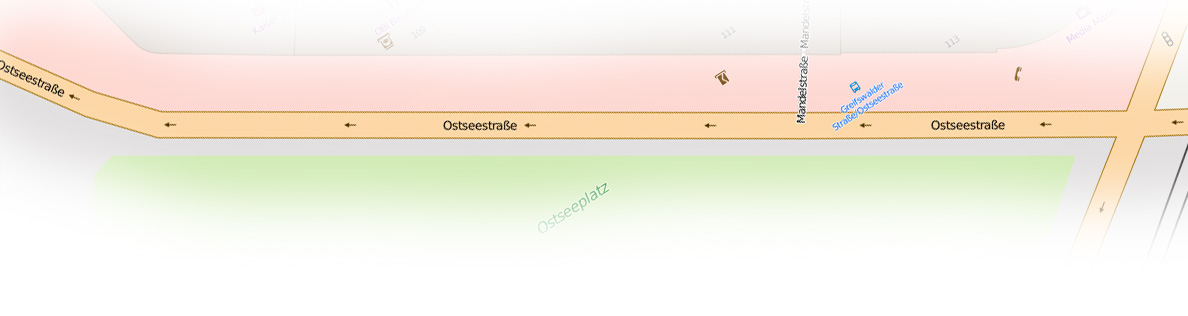
\includegraphics[width=1\textwidth]{gfx/osm_streets_1.jpg}}
   \caption{Teilausschnitt einer Straße aus OpenStreetMap}
   \label{fig:osm_streets_1}
\end{figure}
Die Unterteilung einer Straße in mehrere Ways ist mitunter notwendig, da an einem Way-Element alle Daten des aktuellen Straßenabschnitts, wie z.B. die zulässige Höchstgeschwindigkeit, durch \textit{Tags} gespeichert sind.
Sofern sich diese Daten im Straßenverlauf ändern, wird dies durch ein separates Way-Element wiedergegeben.
Der hier gezeigte Teilabschnitt ist ebenfalls bereits in zwei separate Way-Elemente mit den ID´s \texttt{241186022} und \texttt{4615358} untergliedert (Abbildung \ref{fig:osm_streets_2}).
\begin{figure}[htb]
  \centering
   \fbox{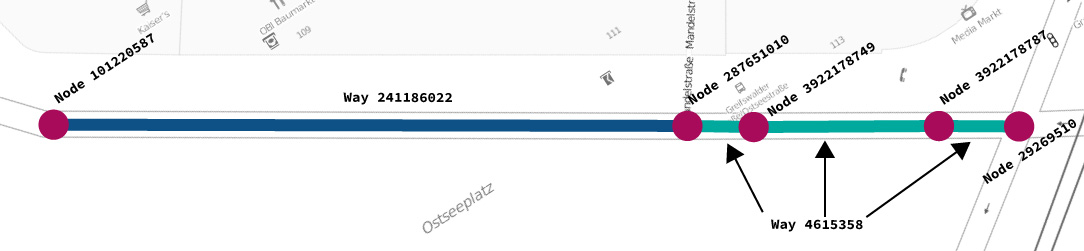
\includegraphics[width=1\textwidth]{gfx/osm_streets_2.jpg}}
   \caption{Beispiel für multiple Ways einer Straße}
   \label{fig:osm_streets_2}
\end{figure}
Dies war notwendig, da sich die Anzahl der Fahrspuren geändert hat.
Der Tag mit dem Key ``lanes'' hat seinen Wert von \texttt{2} auf \texttt{3} geändert. Die Änderung ist im Listing \ref{code:osm_streets} auf Zeile 28 und 45 ersichtlich.
\lstset{
  numbers=left,
  numbersep=5pt,
  caption=Vollständige Daten des Straßenabschnitts,
  label=code:osm_streets
}
\begin{lstlisting}
<node id="101220587" visible="true" version="11" changeset="18256244" timestamp="2013-10-08T22:00:56Z" user="Peter Maiwald" uid="90528" lat="52.5464853" lon="13.4424534"/>
<node id="287651010" visible="true" version="5" changeset="23075493" timestamp="2014-06-22T09:26:32Z" user="atpl_pilot" uid="881429" lat="52.5459138" lon="13.4438910"/>
<node id="3922178749" visible="true" version="1" changeset="36300926" timestamp="2016-01-01T16:28:14Z" user="Balgofil" uid="95702" lat="52.5458508" lon="13.4440518">
 <tag k="bus" v="yes"/>
 <tag k="name" v="Greifswalder Straße/Ostseestraße"/>
 <tag k="public_transport" v="stop_position"/>
 <tag k="ref:BVG" v="105416"/>
 <tag k="website" v="http://qr.bvg.de/h105416"/>
 <tag k="wheelchair" v="limited"/>
</node>
<node id="3922178787" visible="true" version="1" changeset="36300926" timestamp="2016-01-01T16:28:15Z" user="Balgofil" uid="95702" lat="52.5456743" lon="13.4445025">
 <tag k="crossing" v="traffic_signals"/>
 <tag k="highway" v="crossing"/>
</node>
<node id="29269510" visible="true" version="11" changeset="36300926" timestamp="2016-01-01T16:28:39Z" user="Balgofil" uid="95702" lat="52.5456175" lon="13.4446475">
 <tag k="TMC:cid_58:tabcd_1:Class" v="Point"/>
 <tag k="TMC:cid_58:tabcd_1:Direction" v="negative"/>
 <tag k="TMC:cid_58:tabcd_1:LCLversion" v="9.00"/>
 <tag k="TMC:cid_58:tabcd_1:LocationCode" v="21554"/>
 <tag k="TMC:cid_58:tabcd_1:NextLocationCode" v="21555"/>
 <tag k="TMC:cid_58:tabcd_1:PrevLocationCode" v="21553"/>
</node>
<way id="241186022" visible="true" version="4" changeset="35323067" timestamp="2015-11-15T08:45:00Z" user="anbr" uid="43566">
 <nd ref="287651010"/>
 <nd ref="101220587"/>
 <tag k="cycleway" v="lane"/>
 <tag k="highway" v="primary"/>
 <tag k="lanes" v="3"/>
 <tag k="maxspeed" v="50"/>
 <tag k="name" v="Ostseestraße"/>
 <tag k="oneway" v="yes"/>
 <tag k="postal_code" v="10409"/>
 <tag k="ref" v="L 1004"/>
 <tag k="sidewalk" v="right"/>
 <tag k="turn:lanes" v="left|none|none"/>
 <tag k="wikipedia" v="de:Ostseestraße"/>
</way>
<way id="4615358" visible="true" version="27" changeset="36300926" timestamp="2016-01-01T16:28:33Z" user="Balgofil" uid="95702">
 <nd ref="29269510"/>
 <nd ref="3922178787"/>
 <nd ref="3922178749"/>
 <nd ref="287651010"/>
 <tag k="cycleway" v="lane"/>
 <tag k="highway" v="primary"/>
 <tag k="lanes" v="2"/>
 <tag k="maxspeed" v="50"/>
 <tag k="name" v="Ostseestraße"/>
 <tag k="oneway" v="yes"/>
 <tag k="postal_code" v="10409"/>
 <tag k="ref" v="L 1004"/>
 <tag k="sidewalk" v="right"/>
 <tag k="wikipedia" v="de:Ostseestraße"/>
</way>
\end{lstlisting}
\lstset{
  numbers=none,
  caption=,
  label=
  }

\section{Beispiel zur Verwendung von JGraphT zur Trennung eines Graphen in zusammenhängende Elemente}
\label{sec:appendix:jgrapht_separation}
\lstset{
  language=Java,
  numbers=left,
  caption=Beispiel der Trennung eines Graphen in verbundene Teile,
  label=jgrapht_separation,
  keywordstyle=\color{javapurple}\bfseries,
  stringstyle=\color{javared},
  commentstyle=\color{javagreen},
  morecomment=[s][\color{javadocblue}]{/**}{*/},
}
\begin{lstlisting}
import org.jgrapht.UndirectedGraph;
import org.jgrapht.alg.ConnectivityInspector;
import org.jgrapht.graph.DefaultEdge;
import org.jgrapht.graph.SimpleGraph;

// ...
 
// Lege neuen leeren Graphen an, Knoten sind Objekte vom Typ Long
UndirectedGraph<Long, DefaultEdge> graph = new SimpleGraph<>(DefaultEdge.class);
// Graph mit 4 Knoten und 2 Kanten befüllen
Long v1 = new Long(1);
Long v2 = new Long(2);
Long v3 = new Long(3);
Long v4 = new Long(4);
graph.addVertex(v1);
graph.addVertex(v2);
graph.addVertex(v3);
graph.addVertex(v4);
graph.addEdge(v1, v2);
graph.addEge(v3, v4);
// Erzeuge neuen ConnectivityInspector
ConnectivityInspector<Long, DefaultEdge> ci = new ConnectivityInspector<>(graph);
// Erzeuge eine Liste von Sets mit zusammenhängenden Knoten
// Hier werden jetzt zwei Sets erzeugt. (1,2) und (3,4)
List<Set<Long>> connectedNodes = ci.connectedSets(); 
\end{lstlisting}
  
\section{GraphSeparator.java}
\label{sec:appenix:ose:graphseparator}
\lstset{
  language=Java,
  numbers=left,
  label=,
  caption=GraphSeparator.java,
  keywordstyle=\color{javapurple}\bfseries,
  stringstyle=\color{javared},
  commentstyle=\color{javagreen},
  morecomment=[s][\color{javadocblue}]{/**}{*/},
}
\begin{lstlisting}
package de.dfki.OsmosisStreetExtractor.util.geo;

import de.dfki.OsmosisStreetExtractor.util.database.OsmosisDB;
import de.dfki.OsmosisStreetExtractor.util.database.StreetGroup;
import org.jgrapht.UndirectedGraph;
import org.jgrapht.alg.ConnectivityInspector;
import org.jgrapht.graph.DefaultEdge;
import org.jgrapht.graph.SimpleGraph;

import java.util.ArrayList;
import java.util.HashMap;
import java.util.List;
import java.util.Set;

/**
* Created by Tom Oberhauser
* This class is used to separate a whole wayset (i.e. streets) into separate parts
*/
public class GraphSeparator {
  
  private final ArrayList<ArrayList<Long>> clusters_by_name;
  private final ArrayList<ArrayList<Long>> clusters_by_ref;
  private final ArrayList<ArrayList<Long>> clusters_by_intref;
  
  public GraphSeparator(StreetGroup streetGroup, OsmosisDB db) {
    /*
    * graphs for all ways
    */
    UndirectedGraph<Long, DefaultEdge> wayGraphStreetName = new SimpleGraph<>(DefaultEdge.class);
    UndirectedGraph<Long, DefaultEdge> wayGraphStreetRef = new SimpleGraph<>(DefaultEdge.class);
    UndirectedGraph<Long, DefaultEdge> wayGraphStreetIntRef = new SimpleGraph<>(DefaultEdge.class);
    
    /*
    * K: nodeId, V: WayIds (1 to n)
    */
    HashMap<Long, ArrayList<Long>> name_nodeId_2_wayIds = new HashMap<>();
    HashMap<Long, ArrayList<Long>> ref_nodeId_2_wayIds = new HashMap<>();
    HashMap<Long, ArrayList<Long>> intref_nodeId_2_wayIds = new HashMap<>();
    
    /*
    * Populate graph for name
    */
    if (streetGroup.hasName()) {
      populateGraph(wayGraphStreetName, name_nodeId_2_wayIds, db, db.getWaysForStreetName(streetGroup.getName()));
    }
    db.removeStreetName(streetGroup.getName()); //street name has been parsed, remove out of database.
    
    /*
    * Populate graph for ref
    */
    if (streetGroup.hasRef()) {
      populateGraph(wayGraphStreetRef, ref_nodeId_2_wayIds, db, db.getWaysForStreetRef(streetGroup.getRef()));
    }
    db.removeStreetRef(streetGroup.getRef()); //street ref has been parsed, remove out of database.
    
    /*
    * Populate graph for int_ref
    */
    if (streetGroup.hasIntRef()) {
      populateGraph(wayGraphStreetIntRef, intref_nodeId_2_wayIds, db, db.getWaysForStreetIntRef(streetGroup.getIntRef()));
    }
    db.removeStreetIntRef(streetGroup.getIntRef()); //street ref has been parsed, remove out of database.
    
    /*
    * Split graph into parts and generate a List with Sets of NodeIds
    */
    ConnectivityInspector<Long, DefaultEdge> ci_streetName = new ConnectivityInspector<>(wayGraphStreetName);
    List<Set<Long>> connectedNodesByName = ci_streetName.connectedSets();  //separate whole graph into isolated parts
    
    ConnectivityInspector<Long, DefaultEdge> ci_streetRef = new ConnectivityInspector<>(wayGraphStreetRef);
    List<Set<Long>> connectedNodesByRef = ci_streetRef.connectedSets();  //separate whole graph into isolated parts
    
    ConnectivityInspector<Long, DefaultEdge> ci_streetIntRef = new ConnectivityInspector<>(wayGraphStreetIntRef);
    List<Set<Long>> connectedNodesByIntRef = ci_streetIntRef.connectedSets();  //separate whole graph into isolated parts
    
    clusters_by_name = parseGraphClusters(connectedNodesByName, name_nodeId_2_wayIds);
    clusters_by_ref = parseGraphClusters(connectedNodesByRef, ref_nodeId_2_wayIds);
    clusters_by_intref = parseGraphClusters(connectedNodesByIntRef, intref_nodeId_2_wayIds);
  }
  
  /**
  * Takes a list of sets of connected nodeIds and generates lists of lists of connected wayIds
  *
  * @param connectedSets      list of sets of connected nodes
  * @param node2wayDictionary nodeId -> wayId lookup dictionary
  * @return A list of lists which contain all wayIds for one connected set / cluster
  */
  private ArrayList<ArrayList<Long>> parseGraphClusters(List<Set<Long>> connectedSets, HashMap<Long, ArrayList<Long>> node2wayDictionary) {
    ArrayList<ArrayList<Long>> retVal = new ArrayList<>();
    for (Set<Long> aggregate : connectedSets) {
      ArrayList<Long> currentAggregateWays = new ArrayList<>();
      for (Long nodeId : aggregate) {
        for (Long wayId : node2wayDictionary.get(nodeId)) {
          currentAggregateWays.add(wayId);
        }
      }
      retVal.add(currentAggregateWays);
    }
    return retVal;
  }
  
  /**
  * Takes a list of wayIds and populates the graph and the lookup HashMaps
  *
  * @param graph          Graph to populate
  * @param nodeDictionary lookup HashMap to populate (nodeIds -> wayIds)
  * @param db             OsmosisDB object for querying the nodes of ways
  * @param ways           list of way ids
  */
  private void populateGraph(UndirectedGraph<Long, DefaultEdge> graph, HashMap<Long, ArrayList<Long>> nodeDictionary, OsmosisDB db, ArrayList<Long> ways) {
    if (ways != null) { //maybe name got parsed already
      for (Long wayId : ways) {
        ArrayList<Long> nodesArray = db.getNodeIds(wayId); //Get array of nodes for current way
        graph.addVertex(nodesArray.get(0)); //add first vertex
        nodeDictionary.putIfAbsent(nodesArray.get(0), new ArrayList<>()); //generate way dictionary for node if there is none
        nodeDictionary.get(nodesArray.get(0)).add(wayId); //add wayId for node
        for (int i = 1; i < nodesArray.size(); i++) {
          Long currentNode = nodesArray.get(i);
          Long lastNode = nodesArray.get(i - 1);
          graph.addVertex(currentNode);
          if (!currentNode.equals(lastNode)) { //loop detection
            graph.addEdge(lastNode, currentNode);
          }
          nodeDictionary.putIfAbsent(currentNode, new ArrayList<>()); //generate way dictionary for node if there is none
          nodeDictionary.get(currentNode).add(wayId); //add wayId for node
        }
      }
    }
  }
  
  /**
  * Returns all clusters by name
  *
  * @return list of lists of way ids
  */
  public ArrayList<ArrayList<Long>> getClustersByName() {
    return clusters_by_name;
  }
  
  /**
  * Returns all clusters by ref
  *
  * @return list of lists of way ids
  */
  public ArrayList<ArrayList<Long>> getClustersByRef() {
    return clusters_by_ref;
  }
  
  /**
  * Returns all clusters by int_ref
  *
  * @return list of lists of way ids
  */
  public ArrayList<ArrayList<Long>> getClustersByIntref() {
    return clusters_by_intref;
  }
}
\end{lstlisting}

\section{Beispielausgabe der Straßenliste des OsmosisStreetExtractor}
\label{sec:appendix:ose:output}
Es folgt eine Beispielausgabe des \texttt{OsmosisStreetExtractor} in Listing \ref{ose_outputexample}.
Der Inhalt des Feldes \texttt{linestring} wurde aus Gründen der Lesbarkeit gekürzt.
\lstset{
  language=,
  numbers=left,
  caption=Beispielausgabe des OsmosisStreetExtractor,
  label=ose_outputexample,
}
\begin{lstlisting}
"id";"name";"linestring";"geojson"
"0";"An der Rudower Höhe";"0105000020E610000001000...4A40";"{"coordinates":[[[13.5190141,52.4209986],[13.5188694,52.4211964],[13.518082,52.4219104]]],"type":"MultiLineString"}"
\end{lstlisting}

\section{General Transit Feed Specification (GTFS)}
\label{sec:appendix:gtfs_spec}
Auszugsweise findet sich hier eine kurze Übersicht des \textit{General Transit Feed Specification (GTFS)} Formates.
GTFS Daten bestehen aus mehreren Textdateien, welche in einem komprimierten Paket vorliegen.
Eine Übersicht über die benötigten Dateien innerhalb eines GTFS Pakets und deren Inhalt ist in Tabelle \ref{tab:gtfs_files} und Abbildung \ref{fig:gtfs_uml} dargestellt. (vgl. \cite{WEB:Google:gtfs:2016})


\begin{table}[h]
\centering
\caption{Benötigte Dateien innerhalb eines GTFS-Pakets}
\label{tab:gtfs_files}
\begin{tabular}{|l|l|}
\hline
\textbf{Datei}  & \textbf{Inhalt}                         \\ \hline
agency.txt      & Verkehrsunternehmen                     \\ \hline
stops.txt       & Bahnhöfe, Haltestellen                  \\ \hline
routes.txt      & Linien, z.B. eine S-Bahn Strecke        \\ \hline
trips.txt       & eine konkrete Fahrt auf einer Linie     \\ \hline
stop\_times.txt & Abfahrtszeiten pro Fahrt und Bahnhof    \\ \hline
calendar.txt    & Tage, an denen ein Dienst verfügbar ist \\ \hline
\end{tabular}
\end{table}

\begin{figure}[H]
  \centering
   \fbox{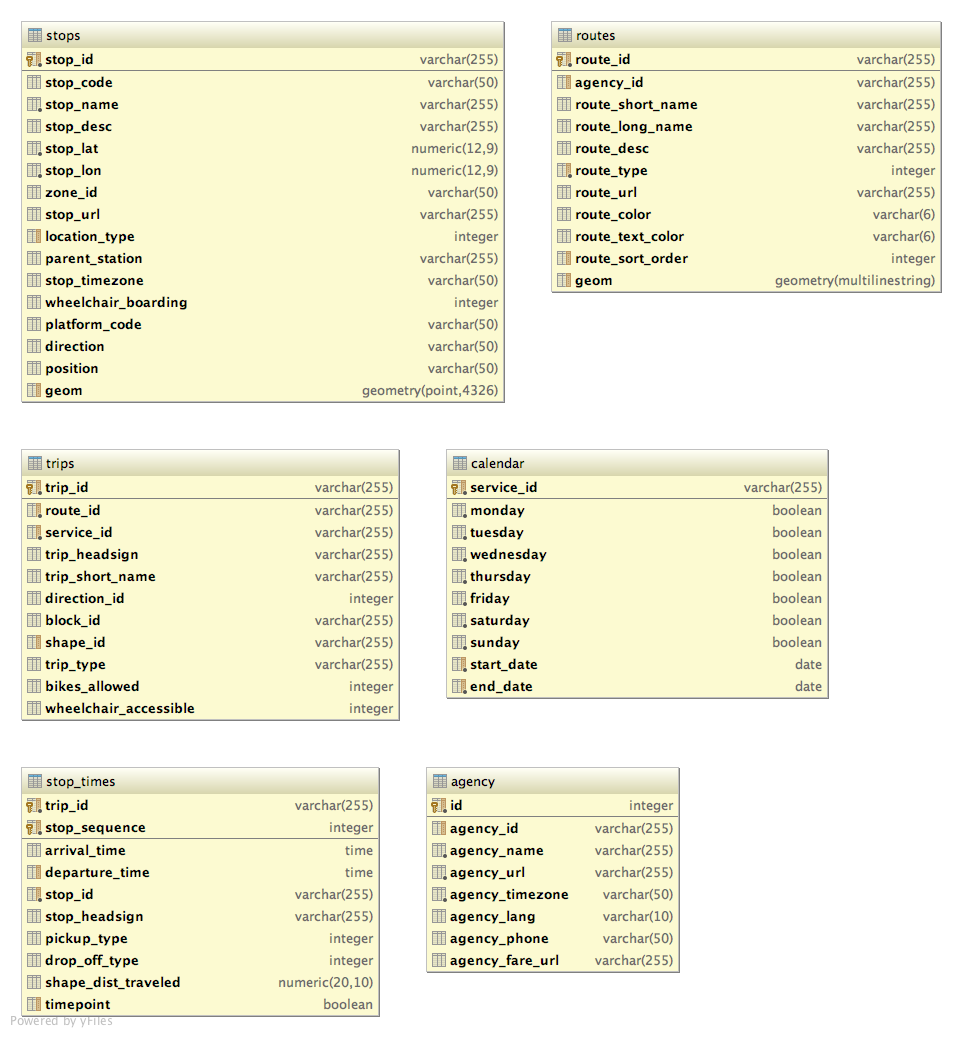
\includegraphics[width=1\textwidth]{gfx/gtfs_uml.png}}
   \caption{Felder innerhalb von GTFS Daten}
   \label{fig:gtfs_uml}
\end{figure}

\section{Levenshtein-Distanz zur Ermittlung der Ähnlichkeit zweier Bahnhofsnamen}
\label{sec:appendix:levenshtein}
Die \textit{Levenshtein-Distanz} zwischen zwei Zeichenketten gibt die Anzahl der Editieroperationen zurück, die notwendig sind um die eine Zeichenkette in die andere zu transformieren.
Der Größe des ermittelten Wertes kann, je nach Länge der Zeichenketten, variieren. 
Die verwendete Bibliothek \textit{java-string-similarity}\footnote{https://github.com/tdebatty/java-string-similarity} bietet die Möglichkeit, eine normalisierte Levenshtein-Distanz zu ermitteln. Dazu wird die ermittelte Levenshtein-Distanz anschließend durch die Länge der längsten Zeichenkette dividiert.
Diese Operation ergibt ein Interval $[0,1]$.

Nun musste ein Algorithmus entwickelt werden, der die normalisierte Levenshtein-Distanz besser auf das Themengebiet Bahnhofsbezeichnungen vorbereitet.
Strings von Bahnhofsbezeichnungen sind zum Beispiel 
\begin{compactitem}
  \item \texttt{''Hauptbahnhof Berlin''}
  \item \texttt{''Berlin Hauptbahnhof''}
\end{compactitem}
Offensichtlich bezeichnen diese den selben Bahnhof, jedoch entspricht die Levenshtein-Distanz zwischen den beiden Zeichenketten $14$ und die normalisierte Levenshtein-Distanz $14/19\approx0,737$.
 
Ich entschied mich dazu, die Zeichenketten vor dem Vergleich zu \textit{tokenizen}, das bedeutet die Zeichenkette anhand bestimmter Trennungszeichen in eine Liste aus Teilzeichenketten aufzuteilen. Dazu wurde die Klasse \texttt{java.util.StringTokenizer} verwendet (Siehe Listing \ref{lev_sum} Zeile 74-81). Anschließend werden die Tokens der beiden zu vergleichenden Zeichenketten alle miteinander verglichen und die jeweils niedrigsten Levenshtein-Distanzen, gewichtet anhand der Länge des kürzeren Tokens aufsummiert (Siehe Listing \ref{lev_sum}). Dies sorgt zum Beispiel dafür, dass die zu Beginn erwähnten Zeichenketten \textit{''Hauptbahnhof Berlin''} und \textit{''Berlin Hauptbahnhof''} eine Distanz von $0$ aufweisen.

\lstset{
  language=Java,
  numbers=left,
  caption=Klasse StringDistance zur Ermittlung der Gleichheit zweier Bahnhofsnamen,
  label=lev_sum,
  keywordstyle=\color{javapurple}\bfseries,
  stringstyle=\color{javared},
  commentstyle=\color{javagreen},
  morecomment=[s][\color{javadocblue}]{/**}{*/},
}
\begin{lstlisting}
package utils;

import com.google.common.collect.HashBasedTable;
import com.google.common.collect.Table;
import info.debatty.java.stringsimilarity.NormalizedLevenshtein;
import info.debatty.java.stringsimilarity.interfaces.NormalizedStringDistance;

import java.util.ArrayList;
import java.util.List;
import java.util.StringTokenizer;

/**
 * Created by Tom Oberhauser
 * Methods for String comparison
 */
public class StringDistance {
  /**
   * Compares two Strings. It returns a weighted sum of the best matching tokens.
   * (eg. "Berlin Hauptbahnhof" and "(Hauptbahnhof) Berlin" would have a distance of 0)
   *
   * @param s1 left String
   * @param s2 right String
   * @return likelihood [0;1] where 0 is equal and 1 is different
   */
  public static double minDistance(final String s1, final String s2) {
    double retVal = 0;
    int n = 0;
    List<String> words_left = tokenize(s1);
    List<String> words_right = tokenize(s2);
    Table<String, String, Double> matcherTable = HashBasedTable.create();
    /*
    compare every left with every right word and fill matcher tables
     */
    for (String wordLeft : words_left) {
      for (String wordRight : words_right) {
        double lev = levenshtein(wordLeft, wordRight);
        matcherTable.put(wordLeft, wordRight, lev);
      }
    }
    /*
    find smallest values and remove corresponding rows and cols until the table is empty
     */
    while (!matcherTable.isEmpty()) {
      String minRow = null;
      String minCol = null;
      Double minVal = Double.MAX_VALUE;
      for (String row : matcherTable.rowKeySet()) {
        for (String col : matcherTable.columnKeySet()) {
          Double currentCell = matcherTable.get(row, col);
          if (currentCell < minVal) {
            minRow = row;
            minCol = col;
            minVal = currentCell;
          }
        }
      }
      if (minRow != null && minCol != null) {
        int minLength = (minRow.length() <= minCol.length()) ? minRow.length() : minCol.length();
        n += minLength;
        retVal += (minVal * (double) minLength);
        matcherTable.row(minRow).clear();
        matcherTable.column(minCol).clear();
      }
    }
    return retVal / n;
  }

  /**
   * Tokenizes a String
   *
   * @param s String
   * @return List of tokens without delimiters
   */
  private static List<String> tokenize(final String s) {
    List<String> list = new ArrayList<>();
    StringTokenizer tokenizer = new StringTokenizer(s, "()[].-,; ", false);
    while (tokenizer.hasMoreTokens()) {
      list.add(tokenizer.nextToken());
    }
    return list;
  }

  /**
   * Calculates the normalized levenshtein distance of two Strings
   *
   * @param s1 left String
   * @param s2 right String
   * @return likelihood [0;1] where 0 is equal and 1 is different
   */
  private static double levenshtein(final String s1, final String s2) {
    NormalizedStringDistance nlv = new NormalizedLevenshtein();
    return nlv.distance(s1, s2);
  }
}
\end{lstlisting}

\section{Kennzahlen zur qualitativen Bewertung eines binären Klassifikators}
\label{sec:appenix:fmeasure}

Ein Klassifikator soll etwas Bestimmtes aus gegebenen Merkmalen vorhersagen.
Genauer gesagt entspricht ein Klassifikator einer Abbildung eines Merkmalsraumes auf eine Menge von Klassen.
Um die Qualität dieser Vorhersage bzw. Abbildung zu bewerten, existieren Kennzahlen.
Im Folgenden wird auf die Kennzahlen \textit{Precision (Genauigkeit)}, \textit{Recall (Trefferquote)} und \textit{F-Maß} zur qualitativen Bewertung eines binären Klassifikators eingegangen.

Zunächst muss ein Datensatz mit bekannten Ergebnissen vorliegen.
Dieser wird auch Gold-Standard genannt.
Anhand des Gold-Standards können nun Vorhersagen mit bekannten Ergebnissen durchgeführt und eine \textit{Wahrheitsmatrix} befüllt werden. In Tabelle \ref{tab:wahrheitsmatrix} ist eine Wahrheitsmatrix für die Beispielklassen \texttt{+} und \texttt{-} abgebildet. 
\begin{table}[]
\centering
\caption{Wahrheitsmatrix}
\label{tab:wahrheitsmatrix}
\begin{tabular}{|l|l|l|}
\hline
\textbf{}           & \textbf{Vorhersage +} & \textbf{Vorhersage -} \\ \hline
\textbf{Wahrheit +} & True Positive ($TP$)    & False Negative ($FN$)   \\ \hline
\textbf{Wahrheit -} & False Positive ($FP$)   & True Negative ($TN$)    \\ \hline
\end{tabular}
\end{table}

Anhand der Messwerte $TP, FP, FN, TN$ lassen sich nun Kennzahlen errechnen.

\subsubsection{Precision (Genauigkeit)}

Der \textit{Precision-Wert} gibt das Verhältnis zwischen allen positiven Vorhersagen und den korrekten positiven Vorhersagen an. Vereinfacht gesagt, wie viele von den positiv vorhergesagten Ergebnissen waren korrekt.

$$Precision = \frac{TP}{TP + FP}$$

\subsubsection{Recall (Trefferquote)}

Der \textit{Recall-Wert} gibt das Verhältnis zwischen allen korrekt als positiv vorhergesagten Objekten zu der Gesamtheit der tatsächlich positiven Objekte an. Vereinfacht gesagt, wie viele positive Ergebnisse wurden wirklich gefunden.
$$Recall = \frac{TP}{TP + FN}$$

\subsubsection{F-Maß}

Die Kennzahlen \textit{Precision} und \textit{Recall} alleine ergeben noch keine gute Abbildung der Vorhersagequalität.
Beispielsweise lässt sich der Precision-Wert anheben, indem der Klassifikator nur ein einzelnes Ergebnis als \texttt{+} korrekt klassifiziert.
Alle als \texttt{+} vorhergesagten Werte wären dann in diesem Fall korrekt.
Aus diesem Grund gibt es das \textit{F-Maß}, welche beide Werte miteinander vereint und als Qualitätskriterium verwendet werden kann.

$$F = 2 * \frac{Precision * Recall}{Precision + Recall}$$

Das in diesem Anhang \ref{sec:appenix:fmeasure} erklärte Wissen wurde mir durch meinen Praktikumsbetreuer Philippe Thomas vermittelt und mit Hilfe von Wikipedia vertieft (vgl. \cite{ wiki:fmeasure}).

\section{Beispielausgabe des GTFS2OSMRailwayLinker}
\label{sec:appendix:gtfs2osm_example}
Der Inhalt des Feldes \texttt{boundingBox} wurde aus Gründen der Lesbarkeit gekürzt.
\lstset{
  language=,
  numbers=left,
  caption=Ausgabe des GTFS2OSMRailwayLinker,
  label=,
}
\begin{lstlisting}
id,name,center,boundingBox,osm_node_ids,gtfs_stop_ids
1456,"Berlin Greifswalder Str",0000000001402AE0E29F9CE8DC404A45231B229B35,000000000300...06C0E47,{3659830181,3876863066,1127967028},{8089011}
\end{lstlisting}

